%
% $File: report.tex
% $Date: Tue Nov 05 11:02:57 2013 +0800
%

\documentclass{article}
\usepackage{fontspec}
\usepackage{zhspacing,url,amsmath,amssymb,verbatim}
\usepackage{pdfpages}
\zhspacing
\usepackage{listings}
\usepackage[hyperfootnotes=false,colorlinks,linkcolor=blue,anchorcolor=blue,citecolor=blue]{hyperref}
\usepackage[backend=biber]{biblatex}
\usepackage{graphicx}
\usepackage{minted}
\usepackage{subfigure}
\usepackage{indentfirst}
\usepackage{cases}
\usepackage{environ}
\usepackage{array}
\usepackage[top=1in, bottom=1in, left=1.25in, right=1.25in]{geometry}
\usepackage{caption}
%\usepackage{tikz}
%\usepackage{dot2texi}

% $File: mint-defs.tex
% $Date: Sun Nov 17 23:37:24 2013 +0800
% $Author: Xinyu Zhou <zxytim@gmail.com>

\newcommand{\inputmintedConfigured}[3][]{\inputminted[fontsize=\footnotesize,
	label=#3,linenos,frame=lines,framesep=0.8em,tabsize=4,#1]{#2}{#3}}

\newcommand{\txtsrc}[2][]{\inputmintedConfigured[#1]{text}{#2}}
\newcommand{\txtsrcpart}[4][]{\txtsrc[firstline=#3,firstnumber=#3,lastline=#4,#1]{#2}}

\newcommand{\cppsrc}[2][]{\inputmintedConfigured[#1]{cpp}{#2}}
\newcommand{\cppsrcpart}[4][]{\cppsrc[firstline=#3,firstnumber=#3,lastline=#4,#1]{#2}}

\newcommand{\javasrc}[2][]{\inputmintedConfigured[#1]{java}{#2}}
\newcommand{\javasrcpart}[4][]{\javasrc[firstline=#3,firstnumber=#3,lastline=#4,#1]{#2}}

\newcommand{\matlabsrc}[2][]{\inputmintedConfigured[#1]{matlab}{#2}}
\newcommand{\matlabsrcpart}[4][]{\matlabsrc[firstline=#3,firstnumber=#3,lastline=#4,#1]{#2}}

\newcommand{\pysrc}[2][]{\inputmintedConfigured[#1]{matlab}{#2}}
\newcommand{\pysrcpart}[4][]{\matlabsrc[firstline=#3,firstnumber=#3,lastline=#4,#1]{#2}}

%\usepackage[T1]{fontenc}
\usepackage{lmodern}
\usepackage{amssymb,amsmath}
\usepackage{ifxetex,ifluatex}
\usepackage{fixltx2e} % provides \textsubscript
% use upquote if available, for straight quotes in verbatim environments
\IfFileExists{upquote.sty}{\usepackage{upquote}}{}
\ifnum 0\ifxetex 1\fi\ifluatex 1\fi=0 % if pdftex
  \usepackage[utf8]{inputenc}
\else % if luatex or xelatex
  \usepackage{fontspec}
  % commented by Xinyu Zhou
  \ifxetex
    \usepackage{xltxtra,xunicode}
  \fi
  \defaultfontfeatures{Mapping=tex-text,Scale=MatchLowercase}
  \newcommand{\euro}{€}
\fi
% use microtype if available
\IfFileExists{microtype.sty}{\usepackage{microtype}}{}
\usepackage{color}
\usepackage{fancyvrb}
\newcommand{\VerbBar}{|}
\DefineShortVerb[commandchars=\\\{\}]{\|}
\DefineVerbatimEnvironment{Highlighting}{Verbatim}{commandchars=\\\{\}}
% Add ',fontsize=\small' for more characters per line
\newenvironment{Shaded}{}{}
\newcommand{\KeywordTok}[1]{\textcolor[rgb]{0.00,0.44,0.13}{\textbf{{#1}}}}
\newcommand{\DataTypeTok}[1]{\textcolor[rgb]{0.56,0.13,0.00}{{#1}}}
\newcommand{\DecValTok}[1]{\textcolor[rgb]{0.25,0.63,0.44}{{#1}}}
\newcommand{\BaseNTok}[1]{\textcolor[rgb]{0.25,0.63,0.44}{{#1}}}
\newcommand{\FloatTok}[1]{\textcolor[rgb]{0.25,0.63,0.44}{{#1}}}
\newcommand{\CharTok}[1]{\textcolor[rgb]{0.25,0.44,0.63}{{#1}}}
\newcommand{\StringTok}[1]{\textcolor[rgb]{0.25,0.44,0.63}{{#1}}}
\newcommand{\CommentTok}[1]{\textcolor[rgb]{0.38,0.63,0.69}{\textit{{#1}}}}
\newcommand{\OtherTok}[1]{\textcolor[rgb]{0.00,0.44,0.13}{{#1}}}
\newcommand{\AlertTok}[1]{\textcolor[rgb]{1.00,0.00,0.00}{\textbf{{#1}}}}
\newcommand{\FunctionTok}[1]{\textcolor[rgb]{0.02,0.16,0.49}{{#1}}}
\newcommand{\RegionMarkerTok}[1]{{#1}}
\newcommand{\ErrorTok}[1]{\textcolor[rgb]{1.00,0.00,0.00}{\textbf{{#1}}}}
\newcommand{\NormalTok}[1]{{#1}}
% \ifxetex
%   \usepackage[setpagesize=false, % page size defined by xetex
%               unicode=false, % unicode breaks when used with xetex
%               xetex]{hyperref}
% \else
%   \usepackage[unicode=true]{hyperref}
% \fi
\hypersetup{breaklinks=true,
            bookmarks=true,
            pdfauthor={},
            pdftitle={},
            colorlinks=true,
            urlcolor=blue,
            %linkcolor=magenta,
            pdfborder={0 0 0}}
%\urlstyle{same}  % don't use monospace font for urls
\setlength{\parindent}{0pt}
\setlength{\parskip}{6pt plus 2pt minus 1pt}
\setlength{\emergencystretch}{3em}  % prevent overfull lines
%\setcounter{secnumdepth}{0}



\newcommand{\figref}[1]{\hyperref[fig:#1]{Figure\ref*{fig:#1}}}
\newcommand{\tableref}[1]{\hyperref[table:#1]{Table\ref*{table:#1}}}
\newcommand{\centerize}[1]{\begin{center} #1 \end{center}}

\newcommand{\cmd}[1]{{\it #1}}
\newcommand{\ccmd}[1]{\centerize{\cmd{#1}}}

\title{Digital Signal Processing: Speaker Recognition \\ Opening Report}
\author{Xinyu Zhou, Yuxin Wu, and Tiezheng Li\\ Tsinghua University}
\date{}

\bibliography{refs.bib}
\begin{document}

\fontsize{11pt}{1.4em}
\setlength{\baselineskip}{1.6em}
\maketitle


\section{Introduction}
A \textbf{Speaker Recognition} tasks can be classified with respect to different criterion:
Text-dependent or Text-independent, Verification (decide whether the person is he claimed to be) or Identification (decide who the person is by its voice).\cite{SRwiki}

Speech is a kind of complicated signal produced as a result of several transformations occurring at different levels: semantic, linguistic and acoustic.
Differences in these transformations may lead to differences in the acoustic properties of the signals.
The recognizability of speaker can be affected not only by the linguistic message
but also the age, health, emotional state and effort level of the speaker.
Background noise and performance of recording device also interfere
the classification process.

Speaker recognition is an important part of Human-Computer Interaction (HCI).
As the trend of employing wearable computer reveals,
Voice User Interface (VUI) has been a vital part of such computer.
As these devices are particularly small, they are more likely to lose and be stolen.
In these scenarios, speaker recognition is not only a good HCI,
but also a combination of seamless interaction with computer and security guard
when the device is lost.
The need of personal identity validation will become more acute in the future.
Speaker verification may be essential in business telecommunications.
Telephone banking and telephone reservation services will develop rapidly
when secure means of authentication were available.

Also,the identity of a speaker is quite often at issue in court cases.
A crime victim may have heard but not seen the perpetrator,
but claim to recognize the perpetrator as someone whose voice was previously familiar;
or there may be recordings of a criminal whose identity is unknown.
Speaker recognition technique may bring a reliable scientific determination.

Furthermore, these techniques can be used in environment which demands high security.
It can be combined with other biological metrics to form a multi-modal authentication system.

In this task, our goal is to build a proof-of-concept text-dependent speaker recognition system with GUI support.
Hopefully, we would like to extend its ability to a text-independent speaker recognition system.

\section{Approach}

Based on weeks of literature reviewing and testing,
we have designed our overall approach to this task as followed:

\begin{enumerate}
    \item Energy-Based VAD

      Input audio signals are very likely to contain significantly large ratio of blank signals.
      VAD (Voice Activity Detector)
      is a preprocessing technique to filter out the blank period.
      The most common approach toward this goal is to use energy-based feature of signals.

      \item Cepstrum-Based Features

        Research showed that cepstrum-based features are more discrimitive in the task of speech and speaker recognition/verification.
        We decide to apply common cepstrum features extraction routine, such as MFCC (Mel-frequency Cepstrum Coefficients), LFCC,
        after the original signals are preprocessed by VAD.

       The basic procedure of MFCC is shown below, and the details about
       extracting MFCC is already been explained in the previous reports.
       The output of this step, is a sequence of fixed-dimension vectors, which will be used later in model training.

      \begin{figure}[H]
        \centering
        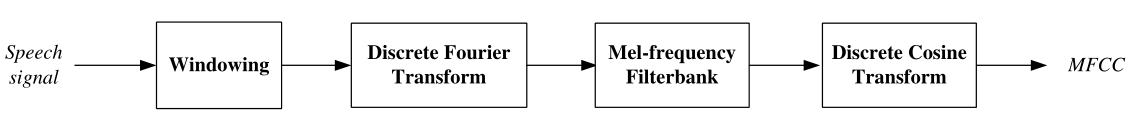
\includegraphics[width=\textwidth]{res/MFCC.png}
      \end{figure}

    \item GMM and UBM Model

      Since the feature vectors of a speaker tend to cluster into \textbf{several} groups
      in the feature space,
      the model of a specific speaker can be well described by using GMM (Gaussian Mixture Model).
      Moreover, for different speakers, the components of their individual GMMs
      will also have similar distributions, which discriminate different syllables.
      Therefore, an UBM (Universal Background Model) can be first trained for all speakers,
      and then we can get adapted GMMs which fit this task better.

      \begin{figure}[H]
        \centering
        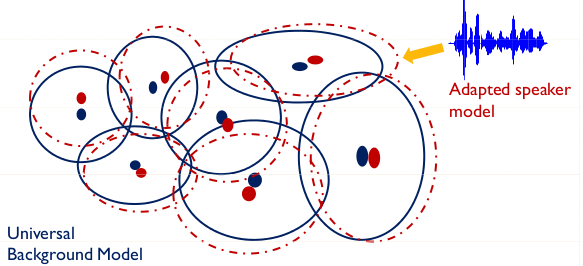
\includegraphics[width=0.7\textwidth]{res/ubm.png}
      \end{figure}

      \item JFA
        GMM-based model can describe the clusterred distribution, but it fails to account for
        different types of variability in each clusterred group.
        However, we only need inter-speaker variability to be modeled,
		but not channel or noise variability. Join Factor Analysis can convey
		such information.

  \end{enumerate}


\printbibliography

\end{document}

